%%%%%%%%%%%%%%%%%%%%%%%%%%%%%%%%%%%%%%%%%%%%%%%%%%%%%%%%%%%%%%%%%%%%%%%%%%%%%%%%
% TUM-Vorlage: Präsentation
%%%%%%%%%%%%%%%%%%%%%%%%%%%%%%%%%%%%%%%%%%%%%%%%%%%%%%%%%%%%%%%%%%%%%%%%%%%%%%%%
%
% Rechteinhaber:
%     Technische Universität München
%     https://www.tum.de
% 
% Gestaltung:
%     ediundsepp Gestaltungsgesellschaft, München
%     http://www.ediundsepp.de
% 
% Technische Umsetzung:
%     eWorks GmbH, Frankfurt am Main
%     http://www.eworks.de
%
%%%%%%%%%%%%%%%%%%%%%%%%%%%%%%%%%%%%%%%%%%%%%%%%%%%%%%%%%%%%%%%%%%%%%%%%%%%%%%%%


%%%%%%%%%%%%%%%%%%%%%%%%%%%%%%%%%%%%%%%%%%%%%%%%%%%%%%%%%%%%%%%%%%%%%%%%%%%%%%%%
% Zur Wahl des Seitenverhältnisses bitte einen der beiden folgenden Befehle
% auskommentieren und den ausführen lassen:
% \documentclass[t]{beamer}
\usepackage[
    orientation=landscape,
    size=custom,
    width=25.4,
    height=19.05,
    scale=0.63 % erzeugt 16pt Schriftgröße
]{beamerposter}

\newcommand{\PraesentationSchriftgroesseSehrGross}{\fontsize{30}{45}}
\newcommand{\PraesentationSchriftgroesseGross}{\fontsize{22}{33}}
\newcommand{\PraesentationSchriftgroesseNormal}{\fontsize{16}{29}}
\newcommand{\PraesentationSchriftgroesseKlein}{\fontsize{12}{18}}
\newcommand{\PraesentationSchriftgroesseDreizeiler}{\fontsize{7}{10}}
\newcommand{\PraesentationSchriftgroesseAufzaehlungszeichen}{\fontsize{10}{8}}

\newcommand{\PraesentationAbstandAbsatz}{22.1pt}
\newcommand{\PraesentationPositionKorrekturOben}{0cm}
\newcommand{\PraesentationBeispieleSchriftgroessen}{30 | 22 | 16 | 12}
\usepackage[utf8]{inputenc}
\usepackage[T1]{fontenc} % Zeichensatzkodierung

\usepackage{calc} % Berechnungen

\usepackage[ngerman, american]{babel} % Deutsche Lokalisierung
\usepackage{graphicx} % Grafiken
\usepackage[absolute, overlay]{textpos} % Positionierung

\usepackage{listings}
\usepackage{lstautogobble}
\usepackage{listings-rust}

% Silbentrennung:
\usepackage{hyphenat}
%\tolerance 2414
%\hbadness 2414
%\emergencystretch 1.5em
%\hfuzz 0.3pt
%\widowpenalty=10000     % Hurenkinder
%\clubpenalty=10000      % Schusterjungen
%\vfuzz \hfuzz

% Euro-Symbol:
\usepackage[gen]{eurosym}
\DeclareUnicodeCharacter{20AC}{\euro{}}

% Schriftart Helvetica:
\usepackage[scaled]{helvet}
\renewcommand{\familydefault}{\sfdefault}

\usepackage{mathptmx} % skalierbare Formelschriften

\usepackage{tabularx}

\usepackage{multicol} % mehrspaltiger Text

\usepackage{tikz}
\usetikzlibrary{arrows, shapes, shapes.multipart, trees, positioning,
    backgrounds, fit, matrix, external}

% Diagramme:
\usepackage{pgfplots}
\pgfplotsset{compat=default}

% Erweiterbare Fusszeile:
\newcommand{\PraesentationFusszeileZusatz}{}

\usepackage{bookmark} % Lesezeichen

% Unterdrückung layoutbedingter Warnungen
\usepackage[immediate]{silence}
\WarningFilter[layout]{lastpage}{Rerun to get the references right} % Gesamtseitenzahl
\WarningFilter[layout]{latex}{Label(s) may have changed.} % Referenz auf letzte Seite
\WarningFilter[layout]{pgfplots}{running in backwards compatibility mode (unsuitable tick labels; missing features).} % Labelerstellung ab Version 1.17 nicht abwärtskompatibel
\WarningFilter[layout]{latex}{There were undefined references}
\WarningFilter[layout]{latex}{Reference `PraesentationDiagramm} % Erstellung einer Legende außerhalb des Diagrammbereichs

% Debugging:
%\DeactivateWarningFilters[layout] % Unterdrückte Warnungen einschalten

\setbeamertemplate{caption}{}

\usepackage{hyperref}
\usepackage{glossaries}

\makeglossaries
\newacronym{abe}{ABE}{Attribute-Based Encryption}
\newacronym{abes}{ABE scheme}{Attribute-Based Encryption scheme}

\newglossaryentry{gls-kgc}
{
        name={key generation center},
        text={Key Generation Center},
        description={Trusted central authority that sets up an \acrshort{abes} and generates keys for users of an \acrshort{abes} }
}

\newglossaryentry{ec}{
  name={elliptic curve},
  text={Elliptic Curve},
  description={Algebraic structure that forms a \gls{group}, see Section~\ref{sec:ec}}
}

\newglossaryentry{group}{
  name={group},
  description={A set together with a binary operation that satisfies the group axioms, see Section~\ref{sec:group}}
}

\newglossaryentry{gls-kp-abe}{
  name={key-policy \acrshort{abe}},
  description={Variant of \gls{abe} where the ciphertext is associated with an \gls{access-policy} and the key is associated with a set of \glspl{attribute}.}
}
\newacronym[see={[Glossary:]{gls-kp-abe}}]{kp-abe}{KP-ABE}{Key-Policy \acrshort{abe}\glsadd{gls-cp-abe}}
\newglossaryentry{gls-cp-abe}{
  name={ciphertext-policy \acrshort{abe}},
  description={Variant of \acrshort{abe} where the key is associated with an \gls{access-policy} and the ciphertext is associated with a set of \glspl{attribute}.}
}
\newacronym[see={[Glossary:]{gls-cp-abe}}]{cp-abe}{CP-ABE}{Ciphertext-Policy \acrshort{abe}\glsadd{gls-cp-abe}}


\newglossaryentry{attribute}{name={attribute},description={Property of an actor or object, e.g. ,,is student'' or ''has blonde hair''}}

\newglossaryentry{access-policy}{
  name={access policy},
  description={A policy that defines what combination of \glspl{attribute} shall be required to access data.}
}

\newglossaryentry{universe}{
  name={attribute universe},
  description={set of possible attributes}
}

\newglossaryentry{small-universe}{
  name={small universe},
  description={type of \acrshort{abe} construction where the possible attributes have to be fixed when the system is instantiated}
}

\newglossaryentry{large-universe}{
  name={large universe},
  description={type of \acrshort{abe} construction where any string can be used as an attribute}
}

\newglossaryentry{pkes}{
  name={asymmetric encryption scheme},
  description={type of encryption scheme where different keys are used for encryption and decryption. The encryption key may be made public, while the decryption key is kept private.}
}

\newglossaryentry{privkes}{
  name={symmetric encryption scheme},
  description={type of encryption scheme where the same key is used for encryption and decryption. This means that the key has to be shared among all parties via some secure channel (e.g. a personal meeting).}
}

\newacronym[see={[Glossary:]{gls-kgc}}]{kgc}{KGC}{Key Generation Center\glsadd{gls-kgc}}
% \newacronym{kgc}{KGC}{Key Generation Center}


% Settings for lstlistings
\lstset{%
  basicstyle=\ttfamily,
  columns=fullflexible,
  autogobble,
  frame=single,
  keywordstyle=\bfseries\color{TUMBlue},
  stringstyle=\color{TUMAccentGreen}
}

\defbeamertemplate{itemize item}{arrow}{\textcolor{TUMOrange}{$\rightarrow$}} % Seitenverhältnis 4:3
%\documentclass[aspectratio=169]{beamer}
\documentclass[t,aspectratio=169]{beamer}
\usepackage[
    orientation=landscape,
    size=custom,
    width=25.4,
    height=14.2875,
    scale=0.5
]{beamerposter}

\newcommand{\PraesentationSchriftgroesseSehrGross}{\fontsize{25}{38}}
\newcommand{\PraesentationSchriftgroesseGross}{\fontsize{18}{27}}
\newcommand{\PraesentationSchriftgroesseNormal}{\fontsize{14}{21}}
\newcommand{\PraesentationSchriftgroesseKlein}{\fontsize{11}{17}}
\newcommand{\PraesentationSchriftgroesseDreizeiler}{\fontsize{7}{10}}
\newcommand{\PraesentationSchriftgroesseAufzaehlungszeichen}{\fontsize{10}{8}}

\newcommand{\PraesentationAbstandAbsatz}{18pt}
\newcommand{\PraesentationPositionKorrekturOben}{-1cm}
\newcommand{\PraesentationBeispieleSchriftgroessen}{25 | 18 | 14 | 11}
\usepackage[utf8]{inputenc}
\usepackage[T1]{fontenc} % Zeichensatzkodierung

\usepackage{calc} % Berechnungen

\usepackage[ngerman, american]{babel} % Deutsche Lokalisierung
\usepackage{graphicx} % Grafiken
\usepackage[absolute, overlay]{textpos} % Positionierung

\usepackage{listings}
\usepackage{lstautogobble}
\usepackage{listings-rust}

% Silbentrennung:
\usepackage{hyphenat}
%\tolerance 2414
%\hbadness 2414
%\emergencystretch 1.5em
%\hfuzz 0.3pt
%\widowpenalty=10000     % Hurenkinder
%\clubpenalty=10000      % Schusterjungen
%\vfuzz \hfuzz

% Euro-Symbol:
\usepackage[gen]{eurosym}
\DeclareUnicodeCharacter{20AC}{\euro{}}

% Schriftart Helvetica:
\usepackage[scaled]{helvet}
\renewcommand{\familydefault}{\sfdefault}

\usepackage{mathptmx} % skalierbare Formelschriften

\usepackage{tabularx}

\usepackage{multicol} % mehrspaltiger Text

\usepackage{tikz}
\usetikzlibrary{arrows, shapes, shapes.multipart, trees, positioning,
    backgrounds, fit, matrix, external}

% Diagramme:
\usepackage{pgfplots}
\pgfplotsset{compat=default}

% Erweiterbare Fusszeile:
\newcommand{\PraesentationFusszeileZusatz}{}

\usepackage{bookmark} % Lesezeichen

% Unterdrückung layoutbedingter Warnungen
\usepackage[immediate]{silence}
\WarningFilter[layout]{lastpage}{Rerun to get the references right} % Gesamtseitenzahl
\WarningFilter[layout]{latex}{Label(s) may have changed.} % Referenz auf letzte Seite
\WarningFilter[layout]{pgfplots}{running in backwards compatibility mode (unsuitable tick labels; missing features).} % Labelerstellung ab Version 1.17 nicht abwärtskompatibel
\WarningFilter[layout]{latex}{There were undefined references}
\WarningFilter[layout]{latex}{Reference `PraesentationDiagramm} % Erstellung einer Legende außerhalb des Diagrammbereichs

% Debugging:
%\DeactivateWarningFilters[layout] % Unterdrückte Warnungen einschalten

\setbeamertemplate{caption}{}

\usepackage{hyperref}
\usepackage{glossaries}

\makeglossaries
\newacronym{abe}{ABE}{Attribute-Based Encryption}
\newacronym{abes}{ABE scheme}{Attribute-Based Encryption scheme}

\newglossaryentry{gls-kgc}
{
        name={key generation center},
        text={Key Generation Center},
        description={Trusted central authority that sets up an \acrshort{abes} and generates keys for users of an \acrshort{abes} }
}

\newglossaryentry{ec}{
  name={elliptic curve},
  text={Elliptic Curve},
  description={Algebraic structure that forms a \gls{group}, see Section~\ref{sec:ec}}
}

\newglossaryentry{group}{
  name={group},
  description={A set together with a binary operation that satisfies the group axioms, see Section~\ref{sec:group}}
}

\newglossaryentry{gls-kp-abe}{
  name={key-policy \acrshort{abe}},
  description={Variant of \gls{abe} where the ciphertext is associated with an \gls{access-policy} and the key is associated with a set of \glspl{attribute}.}
}
\newacronym[see={[Glossary:]{gls-kp-abe}}]{kp-abe}{KP-ABE}{Key-Policy \acrshort{abe}\glsadd{gls-cp-abe}}
\newglossaryentry{gls-cp-abe}{
  name={ciphertext-policy \acrshort{abe}},
  description={Variant of \acrshort{abe} where the key is associated with an \gls{access-policy} and the ciphertext is associated with a set of \glspl{attribute}.}
}
\newacronym[see={[Glossary:]{gls-cp-abe}}]{cp-abe}{CP-ABE}{Ciphertext-Policy \acrshort{abe}\glsadd{gls-cp-abe}}


\newglossaryentry{attribute}{name={attribute},description={Property of an actor or object, e.g. ,,is student'' or ''has blonde hair''}}

\newglossaryentry{access-policy}{
  name={access policy},
  description={A policy that defines what combination of \glspl{attribute} shall be required to access data.}
}

\newglossaryentry{universe}{
  name={attribute universe},
  description={set of possible attributes}
}

\newglossaryentry{small-universe}{
  name={small universe},
  description={type of \acrshort{abe} construction where the possible attributes have to be fixed when the system is instantiated}
}

\newglossaryentry{large-universe}{
  name={large universe},
  description={type of \acrshort{abe} construction where any string can be used as an attribute}
}

\newglossaryentry{pkes}{
  name={asymmetric encryption scheme},
  description={type of encryption scheme where different keys are used for encryption and decryption. The encryption key may be made public, while the decryption key is kept private.}
}

\newglossaryentry{privkes}{
  name={symmetric encryption scheme},
  description={type of encryption scheme where the same key is used for encryption and decryption. This means that the key has to be shared among all parties via some secure channel (e.g. a personal meeting).}
}

\newacronym[see={[Glossary:]{gls-kgc}}]{kgc}{KGC}{Key Generation Center\glsadd{gls-kgc}}
% \newacronym{kgc}{KGC}{Key Generation Center}


% Settings for lstlistings
\lstset{%
  basicstyle=\ttfamily,
  columns=fullflexible,
  autogobble,
  frame=single,
  keywordstyle=\bfseries\color{TUMBlue},
  stringstyle=\color{TUMAccentGreen}
}

\defbeamertemplate{itemize item}{arrow}{\textcolor{TUMOrange}{$\rightarrow$}} % Seitenverhältnis 16:9
%%%%%%%%%%%%%%%%%%%%%%%%%%%%%%%%%%%%%%%%%%%%%%%%%%%%%%%%%%%%%%%%%%%%%%%%%%%%%%%%


%%%%%%%%%%%%%%%%%%%%%%%%%%%%%%%%%%%%%%%%%%%%%%%%%%%%%%%%%%%%%%%%%%%%%%%%%%%%%%%%
%%%%%%%%%%%%%%%%%%%%%%%%%%%%%%%%%%%%%%%%%%%%%%%%%%%%%%%%%%%%%%%%%%%%%%%%%%%%%%%%
% TUM-Vorlage: Personenspezifische Informationen
%%%%%%%%%%%%%%%%%%%%%%%%%%%%%%%%%%%%%%%%%%%%%%%%%%%%%%%%%%%%%%%%%%%%%%%%%%%%%%%%
%
% Rechteinhaber:
%     Technische Universität München
%     https://www.tum.de
% 
% Gestaltung:
%     ediundsepp Gestaltungsgesellschaft, München
%     http://www.ediundsepp.de
% 
% Technische Umsetzung:
%     eWorks GmbH, Frankfurt am Main
%     http://www.eworks.de
%
%%%%%%%%%%%%%%%%%%%%%%%%%%%%%%%%%%%%%%%%%%%%%%%%%%%%%%%%%%%%%%%%%%%%%%%%%%%%%%%%

% Für die Person anpassen:

\newcommand{\PersonTitel}{}
\newcommand{\PersonVorname}{Daniel}
\newcommand{\PersonNachname}{Bücheler}
\newcommand{\PersonStadt}{@Ort@}
\newcommand{\PersonAdresse}{%
    @Adresse@\\%
    @Plz@~\PersonStadt%
}
\newcommand{\PersonTelefon}{@Telefon@}
\newcommand{\PersonFax}{@Fax@}
\newcommand{\PersonEmail}{@E-Mail@}
\newcommand{\PersonWebseite}{@Web@}

\newcommand{\FakultaetAnsprechpartner}{@Ansprechpartner@}
\newcommand{\LehrstuhlName}{Chair of IT Security}

\newcommand{\EinstellungBankName}{Bayerische Landesbank}
\newcommand{\EinstellungBankIBAN}{DE10700500000000024866}
\newcommand{\EinstellungBankBIC}{BYLADEMM}
\newcommand{\EinstellungSteuernummer}{143/241/80037}
\newcommand{\EinstellungUmsatzsteuerIdentifikationsnummer}{DE811193231}

\hyphenation{} % eigene Silbentrennung                    % !!! DATEI ANPASSEN !!!
%%%%%%%%%%%%%%%%%%%%%%%%%%%%%%%%%%%%%%%%%%%%%%%%%%%%%%%%%%%%%%%%%%%%%%%%%%%%%%%%


\tikzset{
    key/.pic={
      \filldraw (2.7,1) coordinate (-name) -- ++(-7, 0) -- ++(-1,-1) -- ++(1, -1) -- ++(0.5, 0.5) -- ++(0.5, -0.5) -- ++(0.75, 0.75) -- ++(0.75, -0.75) -- ++(0.5, 0.5) -- ++(0.5, -0.5) -- ++(1, 1) -- ++(1, -1) -- ++(0.5, 0.5) -- ++(0.5, -0.5) -- ++(0.5, 0) arc (-180+30:180-30:2) -- cycle;
    }
  }
  
  \tikzset{
    lock/.pic={    
      \fill[even odd rule] (-2.5, 0) -- ++(0,3) -- ++(0.5,0) -- ++(0,1) arc (180:0:2) -- ++(0,-1) -- ++(0.5,0) -- ++(0,-3) -- ++(-5, 0) ++(1, 3) -- ++(0,1) arc (180:0:1.5) -- ++(0,-1) -- ++(-3,0);
    }
  }  
  
  \tikzset{
    tree/.pic={    
      \scoped[sibling distance=20, level distance=12, inner sep=1]{
        \tikzstyle{every node}=[fill, circle, draw, anchor=center];
        \tikzstyle{level 2}=[sibling distance=6];
        \fill (0,0.5) node (root) [anchor=south] {} child {node {} child {node {}} child {node {}} child {node {}}} child { node {} child {node {}}};
      };  
    }
  }   
  

\renewcommand{\PersonTitel}{}
\newcommand{\Datum}{\today}

\renewcommand{\PraesentationFusszeileZusatz}{| Bachelor's Thesis | Implementation of ABE in Rust on ARM Cortex M Processors}

\title{Implementation of Attribute-Based Encryption in Rust on ARM Cortex M Processors}
\author{\PersonTitel{} \PersonVorname{} \PersonNachname}
\institute[]{\UniversitaetName \\ \FakultaetName \\ \LehrstuhlName}
\date[\Datum]{Munich, April 7th, 2021}
\subject{Implementation of Attribute-Based Encryption in Rust on ARM Cortex M Processors}

\def\PolynomialSSS(#1){8 + 7 * #1 - 6 * #1^2 + #1 ^ 3}%


%%%%%%%%%%%%%%%%%%%%%%%%%%%%%%%%%%%%%%%%%%%%%%%%%%%%%%%%%%%%%%%%%%%%%%%%%%%%%%%%
%%%%%%%%%%%%%%%%%%%%%%%%%%%%%%%%%%%%%%%%%%%%%%%%%%%%%%%%%%%%%%%%%%%%%%%%%%%%%%%%
% EINSTELLUNGEN
%%%%%%%%%%%%%%%%%%%%%%%%%%%%%%%%%%%%%%%%%%%%%%%%%%%%%%%%%%%%%%%%%%%%%%%%%%%%%%%%

% Allgemein:
\newcommand{\AllgemeinGestalter}{ediundsepp Gestaltungsgesellschaft}
\newcommand{\AllgemeinErsteller}{eWorks GmbH}

% Universität:
\newcommand{\UniversitaetName}{Technical University of Munich}
\newcommand{\UniversitaetAbkuerzung}{TUM}
\newcommand{\UniversitaetWebseite}{www.tum.de}
\newcommand{\UniversitaetLogoBreite}{19mm}
\newcommand{\UniversitaetLogoHoehe}{1cm}

\newcommand{\UniversitaetAdresse}{%
    Arcisstraße~21\\%
    80333~München%
}

% Fakultät:
\newcommand{\FakultaetName}{Department of Informatics}




% Seitenränder:
\newcommand{\SeitenrandOben}{20mm}
\newcommand{\SeitenrandRechts}{20mm}
\newcommand{\SeitenrandLinks}{25mm}
\newcommand{\SeitenrandUnten}{10mm}

% Falzmarken:
\newcommand{\FalzmarkeOben}{87mm}
\newcommand{\FalzmarkeMitte}{148.5mm}
\newcommand{\FalzmarkeUnten}{192mm}
\newcommand{\FalzmarkeBreite}{2mm}
\newcommand{\FalzmarkeDicke}{0.3pt}
\newcommand{\FalzmarkePositionLinks}{7mm}


% Adressfeld:
\newcommand{\AdressfeldHoehe}{45mm}
\newcommand{\AdressfeldBreite}{85mm}
\newcommand{\AdressfeldAbsenderSchriftgroesse}{7.5pt}
\newcommand{\AdressfeldEmpfaengerSchriftgroesse}{11pt}
\newcommand{\AdressfeldEmpfaengerZeilenabstand}{15pt}

% Text:
\newcommand{\TextOben}{77.5mm}
\newcommand{\TextSchriftgroesse}{11pt}
\newcommand{\TextZeilenabstand}{15pt}

% Fusszeile:
\newcommand{\FusszeilePositionOben}{271mm}
\newcommand{\FusszeileBreite}{165mm}
\newcommand{\FusszeileHoehe}{16.5mm}
\newcommand{\FusszeileZwischenabstand}{2mm}
\newcommand{\FusszeileBreiteGross}{44mm}
\newcommand{\FusszeileBreiteKlein}{35.0mm}
\newcommand{\FusszeileSeitennummerAbstand}{7.7mm}
\newcommand{\FusszeileSchriftgroesse}{7.5pt}
\newcommand{\FusszeileZeilenabstand}{8pt}


%%%%%%%%%%%%%%%%%%%%%%%%%%%%%%%%%%%%%%%%%%%%%%%%%%%%%%%%%%%%%%%%%%%%%%%%%%%%%%%%
% DOKUMENT
%%%%%%%%%%%%%%%%%%%%%%%%%%%%%%%%%%%%%%%%%%%%%%%%%%%%%%%%%%%%%%%%%%%%%%%%%%%%%%%%

\usepackage[a4paper,
    top=\SeitenrandOben,
    bottom=\SeitenrandUnten,
    inner=\SeitenrandLinks,
    outer=\SeitenrandRechts,
    foot=\FusszeileHoehe - 1mm,
    head=35mm,
    includefoot
]{geometry}

\textblockorigin{\SeitenrandLinks}{\SeitenrandOben} % Ursprung für Positionierung

% PDF-Einstellungen:
\usepackage{hyperref}
\hypersetup{
    hidelinks,
    pdfauthor={\PersonVorname{} \PersonNachname},
    pdftitle={\Betreff},
    pdfproducer={\AllgemeinErsteller},
    pdfcreator={\AllgemeinGestalter}
}

\renewcommand*{\raggedsignature}{\raggedright}

\makeatletter
    \@setplength{bfoldmarklength}{\FalzmarkeBreite}
    \@setplength{bfoldmarkvpos}{\FalzmarkeUnten}
    \@setplength{firstfoothpos}{\SeitenrandLinks - 2pt}
    \@setplength{firstfootvpos}{\FusszeilePositionOben}
    \@setplength{firstfootwidth}{\FusszeileBreite}
    \@setplength{foldmarkhpos}{\FalzmarkePositionLinks}
    \@setplength{foldmarkthickness}{\FalzmarkeDicke}
    \@setplength{mfoldmarklength}{\FalzmarkeBreite}
    \@setplength{mfoldmarkvpos}{\FalzmarkeMitte}

    \@setplength{refaftervskip}{\TextZeilenabstand}
    \@setplength{refvpos}{\TextOben}
    \@setplength{sigbeforevskip}{\baselineskip}
    \@setplength{sigindent}{0mm}
    \@setplength{subjectaftervskip}{\baselineskip + \baselineskip + 1pt}

    \@setplength{tfoldmarklength}{\FalzmarkeBreite}
    \@setplength{tfoldmarkvpos}{\FalzmarkeOben}
\makeatother

\KOMAoptions{
    fontsize=\TextSchriftgroesse,
    foldmarks=BMpTv,
    firsthead=false,
    backaddress=no,
    addrfield=no,
    fromalign=false
}

\setkomavar{fromname}{\UniversitaetName}
\setkomavar{fromaddress}{\PersonAdresse}
\addtokomafont{backaddress}{\fontsize{\AdressfeldAbsenderSchriftgroesse}{\AdressfeldAbsenderSchriftgroesse}\selectfont}
\addtokomafont{toaddress}{\fontsize{\AdressfeldEmpfaengerSchriftgroesse}{\AdressfeldEmpfaengerZeilenabstand}\selectfont}

\newcommand{\RuecksendeadresseTrenner}{~| \ignorespaces}

\AtBeginLetter{%
    % Logo:
    \begin{textblock*}{\UniversitaetLogoBreite}[1,0](\textwidth, 0cm)%
        \raggedleft%
        
\includegraphics{./Ressourcen/_Bilder/Universitaet_Logo_RGB.pdf}%
    \end{textblock*}%
    \setlength{\baselineskip}{\TextZeilenabstand}%
    \setlength{\parindent}{0mm} % keine Einrückung am Absatzanfang
    \setlength{\parskip}{\baselineskip} % einzeiliger Abstand nach Absätzen
    % Empfängerfenster:
    \begin{textblock*}{\AdressfeldBreite}[0,0](0cm, 15mm)%
        \raggedbottom\raggedright
        \begin{spacing}{.85}%
        {
            \usekomafont{backaddress}%
            \let\\\RuecksendeadresseTrenner% Umdefinieren von "\\" zu "~| "
            \Absender%
        } \\
        \end{spacing}
        \vspace*{5.5pt}
        \usekomafont{toaddress}%
        \EmpfaengerAdresse
    \end{textblock*}
}

\KOMAoptions{refline=dateleft}
\setkomavar{date}{\Datum}
\setkomavar{place}{\PersonStadt}
\setkomafont{subject}{\bfseries}
\setkomavar{subject}{\Betreff}
\setkomavar{signature}{\PersonVorname~\PersonNachname}

%\setkomavar*{enclseparator}{Anlage\vspace{-3em}}

\renewcommand*{\closing}[1]{#1\vspace*{3\baselineskip}\newline\usekomavar{signature}\newline}
\setkomavar{enclseparator}[Anlage]{~}
\renewcommand{\encl}[1]{\newline{}Anlage~#1}

\KOMAoptions{firstfoot=true}
\setkomafont{pagefoot}{\sffamily\fontsize{7.5pt}{8pt}\selectfont}
\renewcommand{\pagemark}{%
\begin{textblock*}{3em}[1,1](\paperwidth - \SeitenrandLinks - \SeitenrandRechts + \FusszeileSeitennummerAbstand + 3mm, \paperheight - \SeitenrandOben - \SeitenrandUnten)%
    \raggedleft\hfill\usekomafont{pagefoot}\thepage\,/\,\pageref*{LastPage}%
\end{textblock*}%
}

\setkomavar{firstfoot}{
    \TabPositions{2em}%
    \begin{minipage}[t][\FusszeileHoehe][t]{\FusszeileBreiteGross}%
        \usekomafont{pagefoot}%
        \textbf{\UniversitaetName}%
        \newline%
        \FakultaetName%
        \newline%
        \LehrstuhlName%
    \end{minipage}%
    \hspace*{\FusszeileZwischenabstand}%
    \begin{minipage}[t][\FusszeileHoehe][t]{\FusszeileBreiteGross}%
        \raggedright\usekomafont{pagefoot}%
        \textbf{\FakultaetAnsprechpartner}\newline%
        \PersonAdresse%
    \end{minipage}%
    \hspace*{\FusszeileZwischenabstand}%
    \begin{minipage}[t][\FusszeileHoehe][t]{\FusszeileBreiteKlein}%
        \raggedright\usekomafont{pagefoot}%
        Tel.\tab{\PersonTelefon}%
        \def\temp{\PersonFax}\ifx\temp\empty%
        \else%
          \newline Fax\tab{\PersonFax}%
        \fi%
        \newline\newline%
        \PersonEmail\newline%
        \href{http://\PersonWebseite}{\PersonWebseite}\newline%
        \href{http://\UniversitaetWebseite}{\UniversitaetWebseite}%
    \end{minipage}%
    \hspace*{\FusszeileZwischenabstand}%
    \begin{minipage}[t][\FusszeileHoehe][t]{\FusszeileBreiteKlein}%
        \raggedright\usekomafont{pagefoot}%
        \EinstellungBankName\newline%
        IBAN-Nr.: \EinstellungBankIBAN\newline%
        BIC: \EinstellungBankBIC\newline%
        Steuer-Nr.: \EinstellungSteuernummer\newline%
        USt-IdNr.: \EinstellungUmsatzsteuerIdentifikationsnummer\newline%
    \end{minipage}%
    \pagemark%
}

\begin{document}
\raggedright
\begin{letter}{}
\opening{\Gruss}

 % !!! NICHT ENTFERNEN !!!
%%%%%%%%%%%%%%%%%%%%%%%%%%%%%%%%%%%%%%%%%%%%%%%%%%%%%%%%%%%%%%%%%%%%%%%%%%%%%%%%


%%%%%%%%%%%%%%%%%%%%%%%%%%%%%%%%%%%%%%%%%%%%%%%%%%%%%%%%%%%%%%%%%%%%%%%%%%%%%%%%
% FOLIENSTIL: Standard
\PraesentationMasterStandard

\PraesentationTitelseite % Fügt die Startseite ein

\begin{frame}[c]
    \frametitle{Table of Contents}
    \tableofcontents[hideallsubsections]
\end{frame}

\section{Introduction}

\begin{frame}[c]
    \frametitle{What did I do?}

    \begin{center}
        \begin{tikzpicture}[brace/.style={decorate, decoration={brace, amplitude=10pt}}, lbl/.style={midway, anchor=south, align=center}]
            \node[align=center, font=\LARGE] (name) at (0, 0) {\textcolor{TUMBlauDunkel}{Implementation} of \textcolor{TUMOrange}{Attribute-Based} \textcolor{TUMGruen}{Encryption} in Rust\\\textcolor{TUMBlauDunkel}{on ARM Cortex M Processors}};
            \onslide<5->{\draw[brace, color=TUMBlauDunkel] (-8.5,1) -- (-3.45,1) node [lbl, yshift=0.5cm] {Implementation of embedded\\ABE library + Evaluation:\\Does this even make\\sense on a small MCU?};}
            \onslide<3->{\draw[brace, color=TUMOrange] (-2.6,1) -- (2.5, 1) node [lbl, yshift=0.5cm] {e.g. for a student:\\``working on thesis''\\``semester count: 6''};}
            \onslide<2->{\draw[brace, color=TUMGruen] (2.75,1) -- (6, 1) node [lbl, yshift=0.5cm] {alternatives: standard\\symmetric and\\asymmetric crypto?!};}
            \onslide<6->{\draw[brace] (6.85, 1) -- (8.5, 1) node [lbl, xshift=0.25cm, yshift=0.5cm] {memory-safety\\guarantees\\built-in! \vphantom{g}};}
            \onslide<4->{\draw[brace, decoration={mirror}, color=TUMBlauDunkel] (-4.75, -1) -- (4.75, -1) node [lbl, yshift=-0.5cm, anchor=north] {Constrained MCUs!};}
        \end{tikzpicture}
    \end{center}
\end{frame}

\section{Background}
\subsection{Attribute-Based Encryption}
\begin{frame}[c]
    \frametitle{Attribute-Based Encryption (ABE) vs. standard encryption}
    \begin{center}
        
\begin{figure} \centering
    \begin{subfigure}{.8\textwidth}
        \begin{tikzpicture}
            \draw[->] (0, 0) node [anchor=east] {m} -- ++(1, 0) node (encrypt) [anchor=west, draw] {Encrypt};
            \path (encrypt.north) -- +(0, 0.3) pic [anchor=west, scale=0.1, red, fill=red] {key};
            \draw[->] (encrypt.east) -- ++(2, 0) node [anchor=south] {c} -- ++(2,0) node (decrypt) [anchor=west, draw] {Decrypt};
            \path (decrypt.north) -- +(0, 0.3) pic [anchor=west, scale=0.1, red, fill=red] {key};
            \draw[->] (decrypt.east) -- ++(1,0) node [anchor=west] {m};
        \end{tikzpicture}
        \caption{Symmetric Encryption: The same key is used for encryption and decryption. This key needs to be kept secret.} \label{fig:keys-symmetric}
    \end{subfigure}
    \\
    \vspace{0.5cm}
    \begin{subfigure}{.8\textwidth}
        \begin{tikzpicture}
            \draw[->] (0, 0) node [anchor=east] {m} -- ++(1, 0) node (encrypt) [anchor=west, draw] {Encrypt};
            \path (encrypt.north) -- +(0, 0.3) pic [anchor=west, scale=0.1, olive, fill=olive] {key};
            \draw[->] (encrypt.east) -- ++(2, 0) node [anchor=south] {c} -- ++(2,0) node (decrypt) [anchor=west, draw] {Decrypt};
            \path (decrypt.north) -- +(0, 0.3) pic [anchor=west, scale=0.1, red, fill=red] {key};
            \draw[->] (decrypt.east) -- ++(1,0) node [anchor=west] {m};
        \end{tikzpicture}
        \caption{Asymmetric Encryption: Different keys for encryption and decryption. Decryption succeeds if and only if the decryption key is exactly the counterpart to the encryption key. Only the decryption key needs to be kept secret.} \label{fig:keys-asymmetric}
    \end{subfigure}
    \\ 
    \vspace{0.5cm}
    \begin{subfigure}{.8\textwidth}
        \begin{tikzpicture}[sibling distance=4mm, level distance=3mm]
            \draw[->] (0, 0) node [anchor=east] {m} -- ++(1, 0) node (encrypt) [anchor=west, draw] {Encrypt};
            
            \scoped{
                \tikzstyle{every node}=[fill, circle, draw, inner sep=0.5mm];
                \tikzstyle{level 2}=[sibling distance=1.5mm];
                \fill[red] (decrypt.north) -- ++(0, 0.7) node [anchor=south] {} child {node {} child {node {}} child {node {}} child {node {}}} child { node {} child {node {}}};
            };
            \draw[->] (encrypt.east) -- ++(2, 0) node [anchor=south] {c} -- ++(2,0) node (decrypt) [anchor=west, draw] {Decrypt};
            \path (encrypt.north) -- +(0, 0.3) node [olive] {$\{A, B, C\}$};
            \draw[->] (decrypt.east) -- ++(1,0) node [anchor=west] {m};
        \end{tikzpicture}
        \caption{\glslink{gls-kp-abe}{Key-Policy Attribute-Based Encryption}: Attributes for encryption, access structure for decryption. Decryption succeeds if and only if the attributes of the ciphertext satisfy the policy embedded in the key.} \label{fig:keys-abe}
    \end{subfigure}
    \\ 
    \vspace{0.5cm}
    \begin{subfigure}{.8\textwidth}
        \begin{tikzpicture}[sibling distance=4mm, level distance=3mm]
            \draw[->] (0, 0) node [anchor=east] {m} -- ++(1, 0) node (encrypt) [anchor=west, draw] {Encrypt};
            
            \scoped{
                \tikzstyle{every node}=[fill, circle, draw, inner sep=0.5mm];
                \tikzstyle{level 2}=[sibling distance=1.5mm];
                \fill[olive] (encrypt.north) -- ++(0, 0.7) node [anchor=south] {} child {node {} child {node {}} child {node {}} child {node {}}} child { node {} child {node {}}};
            };
            \draw[->] (encrypt.east) -- ++(2, 0) node [anchor=south] {c} -- ++(2,0) node (decrypt) [anchor=west, draw] {Decrypt};
            \path (decrypt.north) -- +(0, 0.3) node [red] {$\{A, B, C\}$};
            \draw[->] (decrypt.east) -- ++(1,0) node [anchor=west] {m};
        \end{tikzpicture}
        \caption{\glslink{gls-cp-abe}{Ciphertext-Policy Attribute-Based Encryption}: \Gls{access-policy} for encryption, attributes for decryption. Decryption succeeds if and only if the attributes of the key match the policy embedded in the ciphertext.} \label{fig:keys-abe}
    \end{subfigure}
    \caption[Keys in different classes of encryption schemes]{Keys used for encryption and decryption in different classes of encryption schemes. Red information has to be kept secret, green information may be made publicly available. For the differences between the two types of \acrshort{abe}, see section~\ref{sec:cp-vs-kp}.}
    \label{fig:key-use}
\end{figure}
    \end{center}
\end{frame}

\begin{frame}[c]
    \frametitle{What for?}
    \centering
    % \begin{figure}[h]
    \begin{tikzpicture}[fullnode/.style={draw, minimum width=3.75cm, minimum height=1.25cm, align=center}]
        % \draw (0, 0) node (soc) {Sensor\\(nRF52840 SoC)} |- ++(5, 0) node (gateway) {Gateway\\(Smartphone or Raspberry Pi)};
        \node[fullnode] (soc) {Sensor \\(nRF52840 SoC)};
        \node[fullnode] (gateway) [right=4cm of soc] {Gateway\\(e.g. Smartphone)};
        \node[fullnode] (cloud) [below=1.5cm of gateway] {Cloud\\(e.g. AWS instance)};
        \node[fullnode] (kgc) [below=1.5cm of soc] {Key Generation\\Center};

        \draw[->] (soc) -- (gateway) node [pos=0.5, align=center] {Bluetooth\\Low Energy};
        \draw[<->] (gateway) -- (cloud) node [pos=0.5, align=center] {Internet\\(TCP/IP)};

        \node[fullnode] (user1) [below=1.5cm of kgc] {User 1\\(e.g. Patient)};
        \node[fullnode] (user2) [below=1.5cm of cloud] {User 2\\(e.g. Doctor)};

        % \draw[->] (kgc) -- (gateway) node [pos=0.5] {Internet};
        \draw[->, dotted] (kgc) -- (soc);% node [pos=0.5, align=center] {Key exchanged\\before deployment};
        \draw[->, dotted] (kgc) -- (user1);% node [pos=0.5] {Internet};
        \draw[->, dotted] (kgc) -- (user2);% node [pos=0.5] {Internet};
        \draw[<->] (user1) -- (cloud) node [pos=0.25, sloped, above] {Internet};
        \draw[<->] (user2) -- (cloud) node [pos=0.5] {Internet};

        \node [draw, dashed, fit=(soc) (gateway), inner sep=1mm, label={[anchor=south west]north west:Carried by the patient}] {};
        \node [red, draw, dashed, fit=(gateway) (cloud), inner sep=2mm, label={[red,anchor=south]above:Not trusted}] {};
    \end{tikzpicture}
    % \caption[Simplified use case for our ABE library]{Simplified use case for end-to-end Attribute Based Encryption with encryption on a constrained sensor MCU. The ABE library developed for this thesis runs on the sensor.}
    % \label{fig:system-architecture}
% \end{figure}

    \onslide<3->{\alert{\large $\rightarrow$ No decryption on the MCU!}}
\end{frame}

\begin{frame}[c]
    \frametitle{How to specify Access Policies?}
    \begin{minipage}{.45\textwidth}
        \centering
        {\Large\texttt{professor OR (PhD AND student)}}
    
        \vspace{.5cm}
        \onslide<2->{
        {\Huge $\Downarrow$}
        \vspace{.5cm}
    
        \begin{tikzpicture}[inner/.style={circle}, l/.style={font=\small}]
            \tikzstyle{every node}=[draw];
            \draw (0,0) node[inner] {\only<-2>{$\lor$}\only<3->{1}} child {node[l] {professor}} child {node[inner] {\only<-2>{$\land$}\only<3->{2}} child {node[l] {PhD}} child {node[l] {student}}};
            % \draw (0,0) node {2} child {{node {A}} child {node {1} child {B} child {C}}};
        \end{tikzpicture}}
    \end{minipage}
    \onslide<3->{
    \begin{minipage}{.13\textwidth}
        \centering
        even more powerful!\\
        \vspace{0.5cm}
        {\Huge $\Rightarrow$}
    \end{minipage}}
    \begin{minipage}{.4\textwidth}
    \centering
    \begin{tikzpicture}[xscale=1.2, yscale=1.2, inner/.style={circle}, l/.style={font=\small, align=center}]
        \tikzstyle{every node}=[draw];
        \draw (0,0) node[inner] {2} child {node[l] {itsec}} child {node[l] {netsec}} child {node[inner] {1} child {node[l] {crypto\\lecture}} child {node[l] {crypto\\seminar}}};

    \end{tikzpicture}
\end{minipage}
\end{frame}

% \begin{frame}[c]
%     \frametitle{How to specify Access Policies?}
%     \begin{minipage}{.45\textwidth}
%         \centering
%         test

%         test2
%     \end{minipage}
%     \onslide<3->{
%     \begin{minipage}{.13\textwidth}
%         \centering
%         even more powerful!\\
%         \vspace{0.5cm}
%         {\Huge $\Rightarrow$}
%     \end{minipage}}
%     \begin{minipage}{.4\textwidth}
    \centering
    \begin{tikzpicture}[xscale=1.2, yscale=1.2, inner/.style={circle}, l/.style={font=\small, align=center}]
        \tikzstyle{every node}=[draw];
        \draw (0,0) node[inner] {2} child {node[l] {itsec}} child {node[l] {netsec}} child {node[inner] {1} child {node[l] {crypto\\lecture}} child {node[l] {crypto\\seminar}}};

    \end{tikzpicture}
\end{minipage}
% \end{frame}

% \subsection{Elliptic Curves}

\begin{frame}<1,3-4>[c]
    \frametitle{Bilinear pairings}
    \begin{minipage}{.04\textwidth}
        ~
    \end{minipage}
    \onslide<3->{\begin{minipage}{.25\textwidth}
        Pairing-Based Cryptography:
        \begin{itemize}
            \item Identity-Based Encryption
            \item Three-Way Diffie-Hellman
            \item \alert{Attribute-Based Encryption}
        \end{itemize}
    \end{minipage}}
    \begin{minipage}{0.7\textwidth}\centering
        \begin{tikzpicture}[grp/.style={draw, ellipse}, align=center]
    \node[grp] (g1) at (0,  2) {\Large$\mathbb{G}_1 = \langle P\rangle$ \\(subgroup of\\elliptic curve)};
    \node[grp] (g2) at (0, -2) {\Large$\mathbb{G}_2 = \langle Q\rangle$\\(subgroup of\\elliptic curve)};
    \node[grp] (gt) at (8, 0) {\Large$\mathbb{G}_T$\\(pairing target group,\\not an elliptic curve)};

    \draw[->] (g1.east) to[out=0, in=180] (gt.west);
    \draw[->] (g2.east) to[out=0, in=180] (gt.west);
\end{tikzpicture}  \\
        % \onslide<2>{* requires special pairing-friendly curves}
        \vspace{0.5cm}
    \end{minipage}
    \vspace{0.5cm}
    \centering
    \onslide<4->{\alert{\large$\rightarrow$ very expensive to calculate (\textasciitilde1600\,ms on our MCU)}}

\end{frame}
%%%%%%%%%%%%%%%%%%%%%%%%%%%%%%%%%%%%%%%%%%%%%%%%%%%%%%%%%%%%%%%%%%%%%%%%%%%%%%%%
% FOLIENSTIL: Standard mit Lehrstuhl-, Fakultäts- und Universitätsnamen im
% Kopfbereich links
% \PraesentationMasterKopfzeileDreizeiler


% \PraesentationTitelseite

% \section{Related Research}
% \begin{frame}[c]
%     \frametitle{Overview of Related Research}
%     \begin{center}
%         \begin{tikzpicture}[
        xscale=1.25,
        circ/.style={fill, circle, inner sep=1mm},
        lbl_a/.style={align=center, above},
        year_a/.style={align=center, below, yshift=-0.1cm},
        lbl_b/.style={align=center, below},
        year_b/.style={align=center, above, yshift=0.1cm},
    ]
    \draw[dashed, very thick] (-1,0) -- (0,0) (17.25,0) -- ++(0.75,0);
    \draw[very thick] (0,0) -- (17.25, 0);
    
    \draw (1,0) node [circ] {} node [year_a] {2005} -- ++(0, 1) node [lbl_a] {Fuzzy IBE\\First mention of ABE};

    \draw (2,0) node [circ] {} node [year_b] {2006} -- ++(0, -1) node [lbl_b] {First expressive\\ABE scheme};

    \draw (3,0) node [circ] {} node [year_a] {2007} -- ++(0, 2.5) node [lbl_a] {Pairing implementation\\for PC hardware};

    \draw (7, 0) node [circ] {} node [year_b] {2011} -- ++(0, -1) node [lbl_b] {Pairing implementation\\on 8-bit MCU\\(reduced security level)};
    
    \draw (11,0) node [circ] {} node [year_a] {2015} -- ++(0, 1) node [lbl_a] {Pairing-free\\ABE scheme\\\&\\ABE implementation\\on smartphones};

    \draw (12,0) node [circ] {} node [year_b] {2016} -- ++(0, -1) node [lbl_b] {ABE implementation\\on constrained sensor\\\&\\ABE implementation\\on powerful IoT nodes};

    \draw (15,0) node [circ] {} node [year_a] {2019} -- ++(0, 1) node [lbl_a] {Attack on pairing-\\free ABE};

    \draw[color=TUMOrange] (17, 0) node [circ] {} node [year_b] {2021} -- ++(0, -1) node [lbl_b] {This project};

    % \draw (3,0) node 
\end{tikzpicture}
%     \end{center}
% \end{frame}

\section{Implementation}
\begin{frame}
    \frametitle{Implemented ABE schemes}
    \vspace{2.5cm}
    \begin{columns}[t]\centering
        \column{.49\textwidth}
        \begin{block}{\centering GPSW}
            \centering
            \begin{itemize}
                \item Proposed by Goyal, Pandey, Sahai and Waters in 2006
                \item First expressive ABE scheme
                \item Thoroughly analyzed and frequently implemented / benchmarked
            \end{itemize}
        \end{block}

        \column{.49\textwidth}
        \begin{block}{\centering YCT}
            \centering
            \begin{itemize}
                \item Proposed by Yao, Chen and Tian in 2015 especially for IoT
                \item Does not use bilinear pairing, only single cyclic group
                \item Security of pairing-free ABE is questioned
            \end{itemize}
        \end{block}
        
    \end{columns}
    \center{\alert{\large $\rightarrow$ Both were implemented for analysis on the SoC}}
\end{frame}

\begin{frame}[c]
    \frametitle{Hard- and Software}
    \begin{columns}[c]
        \column{0.5\textwidth}
        \begin{itemize}
            \item nRF52840 SoC: \textcolor{TUMBlau}{64\,MHz} ARM Cortex-M4, \textcolor{TUMBlau}{256\,KB RAM}
            \item Rust programming language: Memory safety guarantees built in!
            \item Pairing and Elliptic Curve Library: \texttt{rabe-bn}\footnotemark
            \item Use of \texttt{core} library and \texttt{heapless} data structures\footnotemark
        \end{itemize}
        
        \column{0.45\textwidth}
        \begin{figure}
            \includegraphics[width=\textwidth]{figures/nrf52840-dk.png}
            \caption{nRF52840 Development Kit, image: \url{https://www.nordicsemi.com/-/media/Images/Products/DevKits/nRF52-Series/nRF52840-DK/nRF52840-DK-promo.png}}
        \end{figure}
    \end{columns}
    \footnotetext[1]{\url{https://github.com/georgbramm/rabe-bn}}
    \footnotetext[2]{\url{https://crates.io/crates/heapless}}
\end{frame}

\begin{frame}[c, fragile]
    \frametitle{Implementation}
    \begin{block}{How to represent access trees without dynamic memory allocation?}
        % Naive implementation:
        \begin{center}
            \begin{minipage}{0.7\textwidth}
                \begin{lstlisting}[caption={Naive implementation (uses standard library)}]
                    enum AccessTree<'a> {
                        Node(u64, std::vec::Vec<AccessTree<'a>>),
                        Leaf(&'a str),
                    }
                \end{lstlisting}
            \begin{lstlisting}[caption={Refined implementation}]
                type AccessTree<'a, 'b> = &'b [AccessNode<'a>];
                enum AccessNode<'a> {
                    Node(u64, heapless::Vec<u8, consts::U16>),
                    Leaf(&'a str),
                }
                \end{lstlisting}
            \end{minipage}
        \end{center}
    \end{block}
\end{frame}

\begin{frame}[c, fragile]
    \frametitle{Implementation}
    \begin{block}{Porting \texttt{rabe-bn} pairing library to the SoC}
        \begin{itemize}
            \item Replace heap data structures by stack-allocated versions
            \item Implementation \verb+core::fmt::Display+ without use of strings
            \item Single pairing consumes about \textonequarter ~of entire RAM!
        \end{itemize} 
    \end{block}
    \pause
    \begin{block}{Common aspects implemented only once}
        \begin{itemize}
            \item Access trees
            \item Hybrid encryption: key derivation and AES-CCM encryption of plaintext
            \item Polynomials over $\mathbb{F}_r$
        \end{itemize}
        % \begin{center}
        %     \alert{\large $\rightarrow$sss }
        % \end{center}
    \end{block}

\end{frame}

\section{Results}
\begin{frame}[c]
    \frametitle{How to evaluate?}
    \begin{minipage}{.59\textwidth}
        Run the algorithms with different numbers of attributes:\\
        ~
        \begin{itemize} 
            \setlength\itemsep{.75em}
            % \item \texttt{Setup}: Number of attributes in the system
            \item \texttt{Encrypt}: Number of attributes associated with ciphertext
            % \item \texttt{KeyGen}: Number of leafs in Access Tree
            \item \texttt{Decrypt}: \begin{itemize}
                \item Timing: Number of leaves in flat access tree
                \item RAM: Depth of perfect binary access tree
            \end{itemize}
        \end{itemize}
    \end{minipage}
    \begin{minipage}{.4\textwidth}
        \begin{figure}
    \begin{tikzpicture}
        \tikzstyle{every node}=[circle, draw];
        \only<1>{
            \tikzstyle{level 1}=[sibling distance=2cm];
            \draw (0,0) node (root) [anchor=south] {4} child {node {A}} child {node {B}} child {node {C}} child {node {D}};
        }
        \only<2>{
            \tikzstyle{level 1}=[sibling distance=1cm];
            \draw (0,0) node (root) [anchor=south] {4} child {node {A}} child {node {B}} child {node {C}} child {node {D}} child {node {E}} child {node {F}} child {node {G}};
        }

            
    \end{tikzpicture}
    \caption*{Flat access tree}
\end{figure}


% \only<1>{\begin{figure}
%     \begin{tikzpicture}
%         \tikzstyle{every node}=[circle, draw];
%         \tikzstyle{level 1}=[sibling distance=3cm, level distance=1cm];
%         \tikzstyle{level 2}=[sibling distance=1.5cm, level distance=1.5cm];
%         \draw (0,0) node (root) [anchor=south] {2} child {node {2} child {node {A}} child  {node {B}}} child {node {2} child {node {C}} child  {node {D}}};
%     \end{tikzpicture}
%     \caption*{Perfect binary access tree (depth 2)}
% \end{figure}}

\begin{figure}
    \begin{tikzpicture}
        \tikzstyle{every node}=[circle, draw];
        \tikzstyle{level 1}=[sibling distance=4cm, level distance=1cm];
        \tikzstyle{level 2}=[sibling distance=2cm, level distance=1.5cm];
        \tikzstyle{level 3}=[sibling distance=1cm, level distance=1.5cm];

        \only<1>{\draw (0,0) node (root) [anchor=south] {2} child {node {2} child {node {A}} child  {node {B}}} child {node {2} child {node {C}} child  {node {D}}};}

        \only<2>{\draw (0,0) node (root) [anchor=south] {2} 
            child {node {2} child { node {2} child {node {A}} child {node {B}}} child {node {2} child {node {C}} child {node {D}}}}
            child {node {2} child { node {2} child {node {D}} child {node {E}}} child { node {2} child {node {F}} child {node {G}}}
        };}
    \end{tikzpicture}
    \caption*{Perfect binary access tree (depth \only<1>{2}\only<2>{3})}
\end{figure}
    \end{minipage}
\end{frame}

\begin{frame}[c]
    \centering
    \frametitle{Results: Timings (overview)}
    \resizebox{!}{.35\textheight}{
        % \begin{figure}[h]
    % \centering
    \begin{minipage}[h]{0.45\textwidth}
        \begin{tikzpicture}
            \begin{axis}[
                title={GPSW Timings -- overview},
                width=\textwidth,
                xlabel={attributes / leaf nodes},
                ylabel={seconds},
                xmin=0, xmax=32,
                ymin=0, ymax=82000000,
                scaled y ticks=base 10:-6,
                ytick scale label code/.code={}, % removes the '\cdot 10^3' label 
                legend pos=north west,
                grid=major,
                grid style=dashed,
                % legend style={nodes={scale=0.65, transform shape}}
            ]
            \addlegendentry{Setup};
            \addplot [color=orange, mark=square] table [x=atts,y=setup,col sep=comma] {../thesis/data/gpsw06-soc.csv};
            \addlegendentry{Encrypt};
            \addplot [color=blue, mark=triangle] table [x=atts,y=enc,col sep=comma] {../thesis/data/gpsw06-soc.csv};
            \addlegendentry{KeyGen};
            \addplot [color=green, mark=o] table [x=atts,y=keygen,col sep=comma] {../thesis/data/gpsw06-soc.csv};
            \addlegendentry{Decrypt};
            \addplot [color=red, mark=+] table [x=atts,y=dec,col sep=comma] {../thesis/data/gpsw06-soc.csv};
            \end{axis}
        \end{tikzpicture}
    \end{minipage}%
    \begin{minipage}{0.049\textwidth}
        ~
    \end{minipage}
    \begin{minipage}[h]{0.45\textwidth}
        \begin{tikzpicture}
            \begin{axis}[
                title={YCT Timings -- overview},
                width=\textwidth,
                xlabel={attributes / leaf nodes},
                ylabel={seconds},
                xmin=0, xmax=32,
                ymin=0, ymax=11500000,
                scaled y ticks=base 10:-6,
                ytick scale label code/.code={}, % removes the '\cdot 10^3' label 
                legend pos=north west,
                grid=major,
                grid style=dashed,
                % legend style={nodes={scale=0.65, transform shape}}
            ]
            \addlegendentry{Setup};
            \addplot [color=orange, mark=square] table [x=atts,y=setup,col sep=comma] {../thesis/data/yct14-soc.csv};
            \addlegendentry{Encrypt};
            \addplot [color=blue, mark=triangle] table [x=atts,y=enc,col sep=comma] {../thesis/data/yct14-soc.csv};
            \addlegendentry{KeyGen};
            \addplot [color=green, mark=o] table [x=atts,y=keygen,col sep=comma] {../thesis/data/yct14-soc.csv};
            \addlegendentry{Decrypt};
            \addplot [color=red, mark=+] table [x=atts,y=dec,col sep=comma] {../thesis/data/yct14-soc.csv};
            \end{axis}
        \end{tikzpicture}
    \end{minipage}%
%     \caption{Timings of GPSW operations on the SoC.}
%     \label{fig:abe-performance-diagrams-gpsw}
% \end{figure}
    }
\end{frame}

\begin{frame}[c]
    \centering
    \frametitle{Results: Timings (same scale)}
    \resizebox{!}{.35\textheight}{
        
    \begin{minipage}[h]{0.45\textwidth}
        \begin{tikzpicture}
            \begin{axis}[
                title={GPSW Timing},
                width=\textwidth,
                xlabel={attributes / leaf nodes},
                ylabel={seconds},
                xmin=0, xmax=32,
                ymin=0, ymax=10000000,
                scaled y ticks=base 10:-6,
                ytick scale label code/.code={}, % removes the '\cdot 10^3' label 
                legend pos=south east,
                grid=major,
                grid style=dashed,
                % legend style={nodes={scale=0.65, transform shape}}
            ]
            % \addlegendentry{Setup};
            % \addplot [color=orange, mark=square] table [x=atts,y=setup,col sep=comma] {../thesis/data/gpsw06-soc.csv};
            \addlegendentry{Encrypt};
            \addplot [color=blue, mark=triangle] table [x=atts,y=enc,col sep=comma] {../thesis/data/gpsw06-soc.csv};
            % \addlegendentry{KeyGen};
            % \addplot [color=green, mark=o] table [x=atts,y=keygen,col sep=comma] {../thesis/data/gpsw06-soc.csv};
            \addlegendentry{Decrypt};
            \addplot [color=red, mark=+] table [x=atts,y=dec,col sep=comma] {../thesis/data/gpsw06-soc.csv};
            \end{axis}
        \end{tikzpicture}
        
    \end{minipage}%
    \begin{minipage}{0.049\textwidth}
        ~
    \end{minipage}
    \begin{minipage}[h]{0.45\textwidth}
        \begin{tikzpicture}
            \begin{axis}[
                title={YCT Timings},
                width=\textwidth,
                xlabel={attributes / leaf nodes},
                ylabel={seconds},
                xmin=0, xmax=32,
                ymin=0, ymax=10000000,
                scaled y ticks=base 10:-6,
                ytick scale label code/.code={}, % removes the '\cdot 10^3' label 
                grid=major,
                grid style=dashed,
                legend pos=north west,
                % legend style={nodes={scale=0.65, transform shape}}
            ]
            % \addlegendentry{Setup};
            % \addplot [color=orange, mark=square] table [x=atts,y=setup,col sep=comma] {../thesis/data/yct14-soc.csv};
            \addlegendentry{Encrypt};
            \addplot [color=blue, mark=triangle] table [x=atts,y=enc,col sep=comma] {../thesis/data/yct14-soc.csv};
            % \addlegendentry{KeyGen};
            % \addplot [color=green, mark=o] table [x=atts,y=keygen,col sep=comma] {../thesis/data/yct14-soc.csv};
            \addlegendentry{Decrypt};
            \addplot [color=red, mark=+] table [x=atts,y=dec,col sep=comma] {../thesis/data/yct14-soc.csv};
            \end{axis}
        \end{tikzpicture}
    \end{minipage}%

    }
\end{frame}

\begin{frame}[c]
    \frametitle{Results: RAM use}
    \centering
    \begin{minipage}{\textwidth}\centering
    \begin{tikzpicture}
        \begin{axis}[
            % title={RAM use during decryption},
            height=.7\textheight,
            xlabel={depth of the \gls{access-tree}},
            ylabel={kilobytes},
            xmin=0.75, xmax=4.25,
            ymin=0, ymax=360000,
            xtick=data,
            scaled y ticks=base 10:-3,
            ytick scale label code/.code={}, % removes the '\cdot 10^3' label 
            legend pos=north west,
            grid=major,
            minor y tick num=1,
            grid style=dashed,
            legend style={nodes={scale=.8, transform shape}}
        ]
        \addlegendentry{GPSW Dec};
        \addplot [color=blue, mark=o] table [x=layers,y=gpsw-dec,col sep=comma] {../thesis/data/ram.csv};
        \addlegendentry{YCT Dec};
        \addplot [color=orange, mark=triangle] table [x=layers,y=yct-dec,col sep=comma] {../thesis/data/ram.csv};
        \addlegendentry{GPSW Enc};
        \addplot [color=blue, mark=none] {83560};
        \addlegendentry{YCT Enc};
        \addplot [color=orange, mark=none] {22616};
        \addplot [color=black, dashed, mark=none] {256000};
    \end{axis}
    \end{tikzpicture}
\end{minipage}
\end{frame}

\begin{frame}[t]
    \frametitle{Discussion of the results}
    \centering
    \vspace{1.5cm}
    \begin{columns}[t]
        \column{.49\textwidth}
        \begin{block}{\centering GPSW}
            \begin{itemize}
                \item Encryption takes up to 8.5\,s, decryption up to 80\,s
                \item RAM shortage puts hard limit on policy size (two levels), even if using \textbf{entire} available RAM!
            \end{itemize}
        \end{block}
        \column{.49\textwidth}
        \begin{block}{\centering YCT}
            \begin{itemize}
                \item Encryption takes up to 5\,s, decryption up to 12\,s
                \item No issues with RAM use
                \item Possibly worse security than GPSW (without pairings)
            \end{itemize}
        \end{block}
    \end{columns}
    \vspace{0.5cm}
    \begin{minipage}{.5\textwidth}
        \begin{itemize}
            \color{TUMOrange}
            \setbeamertemplate{itemize item}[arrow]
            \item<2-> ABE operations require considerable portion of resources
            \item<3-> YCT scheme without pairings has much better performance
            % \item<4-> Encryption is feasible with both, decryption only with YCT
        \end{itemize}
    \end{minipage}
\end{frame}

\begin{frame}[c]
    \frametitle{Possible improvements?}

    \begin{itemize}
        \pause \item Better performance of pairing library \pause \alert{$\rightarrow$ some libraries in literature do better}
        \pause \item Re-use the AES key \pause \alert{$\rightarrow$ did this for integration, but it's cheating \smiley}
        \pause \item Implement schemes with revocation, delegation, multi-authority ABE ... \pause \alert{$\rightarrow$ Future work!}
    \end{itemize}
    

\end{frame}

\section{Conclusion}
\begin{frame}[c]
    \frametitle{Summary \& Key Takeaways}
    
    % \begin{minipage}{.49\textwidth}        
        For the thesis, I $\dots$

        \pause
        $\dots$ present the mechanisms behind ABE \textcolor{TUMGruen}{\checkmark} \pause \alert{$\rightarrow$ ABE is suited to improve access control in many scenarios!}

        \pause $\dots$ ported the \texttt{rabe-bn} pairing library to the SoC \textcolor{TUMGruen}{\checkmark} \pause \alert{$\rightarrow$ pairing computation works on the SoC, but is still demanding}\\
        \pause \phantom{$\dots$ ported the \texttt{rabe-bn} pairing library to the SoC \textcolor{TUMGruen}{\checkmark}} \alert{$\rightarrow$ RAM is bottleneck for pairing-based implementations}

        \pause $\dots$ built a bare-metal implementation of two ABE schemes \textcolor{TUMGruen}{\checkmark} \pause \alert{$\rightarrow$ programming without OS is doable, but challenging \smiley}

        \pause $\dots$ evaluated their performance on a Cortex-M4 SoC \textcolor{TUMGruen}{\checkmark} \pause \alert{$\rightarrow$ ABE is feasible but remains very expensive}\\        
        \pause \phantom{$\dots$ evaluated their performance on a Cortex-M4 SoC \textcolor{TUMGruen}{\checkmark}} \alert{$\rightarrow$ Encryption works with pairing-free and pairing-based schemes}\\
        \pause \phantom{$\dots$ evaluated their performance on a Cortex-M4 SoC \textcolor{TUMGruen}{\checkmark}} \alert{$\rightarrow$ Decryption with pairing-based scheme not practically feasible \frownie}


    % \end{minipage}
    % \begin{minipage}{.49\textwidth}
    %     Key Takeaways$\dots$\\
    %     $\dots$ ABE is suited for many applications because of its great flexibility\\
    %     $\dots$ ABE is feasible on Cortex-M4 SoCs but remains expensive\\
    %     $\dots$ Many use cases only require encryption on the SoC, which is much easier\\
    %     $\dots$ Bilinear pairings remain a big hurdle and pairing-free schemes can present alternatives (if secure)
    % \end{minipage}
\end{frame}

\PraesentationMasterWeissBlau
\begin{frame}[c]
    \begin{center}
        \Huge Thank you!\\

        \vfill
        \Large Do you have any questions?
    \end{center}
\end{frame}


\PraesentationMasterStandard

\begin{frame}[c]
    \frametitle{ABE interaction overview}
    \begin{figure}
    \centering
    \begin{subfigure}[t]{0.45\textwidth}
        \centering
        \begin{tikzpicture}[actor/.style={draw, minimum width=1.5cm}]
            \node[actor] (a) at (-1,0) {Alice};
            \node[actor] (b) at (1,0) {Bob};
            \node[actor] (kgc) at (0,1.5) {KGC};
        
            \node[above, align=center] at (kgc.north) {$\{PK, MK\}:=\text{Setup}()$};

            \node[below, align=center] at (a.south) {$\{m, \omega\}$\\};
            \node[below, align=center] at (b.south) {$\{\}$};

            \draw[->] (a) -- (kgc) node (lbl_a) [pos=0.5, left, olive] {$S_A$};
            \draw (lbl_a.west) +(-0.25,0) pic [scale=0.5, olive] {tree};

            \draw[->] (b) -- (kgc) node (lbl_b) [pos=0.5, right, blue] {$S_B$};
            \draw (lbl_b.east) +(0.25,0) pic [scale=0.5, blue] {tree};

        \end{tikzpicture}
        \caption{Setup phase I: Generation of parameters}
    \end{subfigure}
    ~~
    \begin{subfigure}[t]{0.45\textwidth}
        \centering
        \begin{tikzpicture}[actor/.style={draw, minimum width=1.5cm}]
            \node[actor] (a) at (-1,0) {Alice};
            \node[actor] (b) at (1,0) {Bob};
            \node[actor] (kgc) at (0,1.5) {KGC};

            \node[above, align=center] at (kgc.north) {$\{PK, MK\}$\\$\textcolor{olive}{k_A} := \text{KeyGen}(PK, MK, \textcolor{olive}{S_A})$\\$\textcolor{blue}{k_B} := \text{KeyGen}(PK, MK, \textcolor{blue}{S_B})$};

            \node[below, align=center] at (a.south) {{\{$PK$, $\textcolor{olive}{k_A}$\}}\\$\{m, \omega\}$};
            \node[below, align=center] at (b.south) {\{$PK$, $\textcolor{blue}{k_B}$\}};

            \draw[->] (kgc) -- (a) node (lbl_a) [pos=0.5, left] {\{$PK$, $\textcolor{olive}{k_A}$\}};
            \draw (lbl_a.north) +(0.35,0) pic [scale=0.05, olive] {key};
            \draw[->] (kgc) -- (b) node (lbl_b) [pos=0.5, right] {\{$PK$, $\textcolor{blue}{k_B}$\}};
            \draw (lbl_b.north) +(0.35,0) pic [scale=0.05, blue] {key};

            % \draw[->] (kgc) edge node [left] {\{$PK$, $\textcolor{olive}{k_A}$\}} (a);
            % \draw[->] (kgc) edge node [right] {\{$PK$, $\textcolor{blue}{k_B}$\}} (b);

        \end{tikzpicture}
        \caption{Setup phase II: Issuing of keys}
    \end{subfigure}
    % \begin{minipage}{0.01\textwidth}
    %     ~
    % \end{minipage}
    % \begin{minipage}[bt][][c]{0.35\textwidth}
    %     \centering
    %     \begin{tikzpicture}[matrixstyle/.style={
    %         matrix of nodes,
    %         nodes in empty cells,
    %         column sep      = 0mm,
    %         row sep         = 2mm,
    %         draw,
    %         nodes={
    %             inner sep=1mm,outer sep=1mm,
    %             minimum size=5mm,
    %             anchor=center,
    %             text centered,
    %             text width=1cm,
    %             execute at begin node={\small\setlength{\baselineskip}{1em}} % WTF.. see https://tex.stackexchange.com/questions/223065/how-to-increase-line-spacing-in-tikz-node
    %         }
    %     }]
    %         \matrix (m) [matrixstyle] at (0,0) {
    %             $PK$ & \node[align=left, text width=3.5cm] {Public Key (same\\for all participants)};\\
    %             $MK$ & \node[align=left, text width=3.5cm] {Master Secret (known\\only to the \acrshort{kgc})};\\
    %             $k_A, k_B$ & \node[align=left, text width=3.5cm] {Private\\Decryption Keys};\\
    %             $S_A, S_B$ & \node[align=left, text width=3.5cm] {Access Structures};\\
    %             $m$ & \node[align=left, text width=3.5cm] {Plaintext message};\\
    %             $\omega$ & \node[align=left, text width=3.5cm] {Set of attributes};\\
    %         };
    %     \end{tikzpicture}
    % \end{minipage}
\end{figure}
\end{frame}

\begin{frame}[c]
    \frametitle{ABE interaction overview}
    \begin{figure}
        \begin{subfigure}[t]{.5\textwidth}
            \addtocounter{subfigure}{2}
            \centering
            \begin{tikzpicture}[actor/.style={draw, minimum width=1.5cm}]
                \node[actor] (a) at (-2,0) {Alice};
                \node[actor] (b) at (2,0) {Bob};
                \node[actor] (kgc) at (0,1.5) {KGC};
            
                \node[above, align=center] at (kgc.north) {$\{PK, MK\}$};

                \node[below, align=center] at (a.south) {{\{$PK$, $\textcolor{olive}{k_A}$\}}\\$\{m, \omega\}$\\$\textcolor{red}{c}:=\text{Encrypt}(PK, m, \omega)$};
                \node[below, align=center] at (b.south) {\{$PK$, $\textcolor{blue}{k_B}$\}\\$m:=\text{Decrypt}(\textcolor{red}{c},\textcolor{blue}{k_B})$};
                % \node[below, align=center] at (a.south) {$\{PK, k_{A}\}$\\$\{m, \omega\}$};;
                % \node[below, align=center] at (b.south) {$\{PK, k_{B}\}$\\$m:=\text{Decrypt}(c,k_B)$};

                \draw[->] (a) edge node (c) [above] {$\textcolor{red}{c}$} (b);

                % \draw[->] (c.north) -- ++(0,.2) node [anchor=south] {\small $\omega$};
            \end{tikzpicture}
            \caption{Exchange of encrypted messages without involvement of the KGC}
        \end{subfigure}
\end{figure}
\end{frame}


\begin{frame}<100>[c]
    \frametitle{ABE scheme: Algorithms}
    \begin{minipage}[t]{0.49\textwidth}
        \begin{center}
            \begin{tikzpicture}[baseline=(current bounding box.north)]
                \node[draw, font=\LARGE] at (0,0) {KGC};
            \end{tikzpicture}
        \end{center}
        \vspace{0.5cm}
        \begin{block}<2->{\centering $(PK, MK) = \text{Setup}(U)$}
            \centering
            Sets up the system and defines the attributes.
            % \begin{itemize}
            %     \item Input: Attribute Universe $U$
            %     \item Output: Public Key $PK$, Master Key $MK$
            % \end{itemize}
        \end{block}
        \vspace{0.5cm}
        \begin{block}<3->{\centering $k = \text{KeyGen}(MK, S)$}
            \centering
            Issues a decryption key under a given access policy.
            % \begin{itemize}
            %     \item Input: Master Key $MK$, Access Policy $S$
            %     \item Ouptut: Decryption key $k$
            % \end{itemize}
        \end{block}
    \end{minipage}
    \begin{minipage}[t]{0.49\textwidth}
        \begin{center}
            \begin{tikzpicture}[baseline=(current bounding box.north)]
                \node[draw, font=\LARGE] at (-1.25,0) (a) {Alice};
                \node[draw, font=\LARGE] at (1.25,0) (b) {Bob};
                \path (a) -- (b) node[pos=0.5, font=\LARGE] {\&};
            \end{tikzpicture}
        \end{center}
        \vspace{0.5cm}
        \begin{block}<4->{\centering $c = \text{Encrypt}(PK, m, \omega)$}
            \centering
            Encrypts plaintext under given list of attributes.
            % \begin{itemize}
            %     \item Input: Attribute Universe $U$
            %     \item Output: Public Key $PK$, Master Key $MK$
            % \end{itemize}
        \end{block}
        \vspace{0.5cm}
        \begin{block}<5->{\centering $m = \text{Decrypt}(k, c)$}
            \centering
            Decrypts ABE ciphertext.
            % \begin{itemize}
            %     \item Input: Master Key $MK$, Access Policy $S$
            %     \item Ouptut: Decryption key $k$
            % \end{itemize}
        \end{block}
    \end{minipage}
\end{frame}

\subsection{Secret Sharing}
\begin{frame}<10>[c]
    \frametitle{Shamir's Threshold Secret Sharing}
    \begin{minipage}{.5\textwidth}
        \begin{itemize}
            \item<1-> Goal: Share a secret $s$
            \begin{itemize}
                \item among $n$ participants
                \item reconstruction possible if $k$ or more shares combined
            \end{itemize}
            \item<2-> Secret shares = points on polynomial
            \item<3-> Reconstruction: Lagrange interpolation
        \end{itemize}
    \end{minipage}
    \begin{minipage}{.48\textwidth}
        \begin{figure}
    \centering
    \begin{tikzpicture}
        \begin{axis} [axis lines=center, xlabel=$x$, ylabel=$p(x)$, ymin=0]
            \addplot [domain=-0.1:5.05, smooth, thick, color=red] { \PolynomialSSS(x)};
            \fill (axis cs:0,\PolynomialSSS(0)) circle [radius=2pt] node [right] {(0,~s)};
            \fill[color=ForestGreen] (axis cs:1,\PolynomialSSS(1)) circle [radius=2pt] node [right] {(1,~10)};
            \fill[color=ForestGreen] (axis cs:2,\PolynomialSSS(2)) circle [radius=2pt] node [right] {(2,~6)};
            \fill[color=ForestGreen] (axis cs:3,\PolynomialSSS(3)) circle [radius=2pt] node [above] {(3,~2)};
            \fill[color=ForestGreen] (axis cs:4,\PolynomialSSS(4)) circle [radius=2pt] node [right] {(4,~4)};
            \fill[color=ForestGreen] (axis cs:5,\PolynomialSSS(5)) circle [radius=2pt] node [left] {(5,~18)};
          \end{axis}
    \end{tikzpicture}
    \caption[Plot of $(5,4)$-threshold secret sharing scheme]{
        Example for a $(5, 4)$-threshold scheme with $s=8$ and $p(x) = 8 + 7x - 6x^2 + x^3$.
        The five green-colored points are distributed as the secret shares.
        As $p(x)$ has degree three, at least four shares are required to reconstruct $s$.
    }
    \label{fig:sss}
\end{figure}
    \end{minipage}
\end{frame}

\begin{frame}
    \frametitle{Secret Sharing down the Access Tree}
    \begin{figure}
    \centering
    \begin{tikzpicture}
        \scoped{
                \tikzstyle{every node}=[circle, draw];
                \draw (0,0) node (root) [anchor=south] {2} child [red] {node (a) {A}} child [red] {node (b) {B}} child [red] {node (subroot) {1} child [blue] {node (c) {C}} child [blue] {node (d) {D}}};
            };
            \path[red] (root) -- +(0, -0.75) node {$p_1(x)$};
            \path[red] (a) -- +(0, -0.5) node {\tiny$p_1(1)$};
            \path[red] (b) -- +(0, -0.5) node {\tiny$p_1(2)$};
            \path[red] (subroot) -- +(0, 0.5) node {\tiny$p_1(3)$};

            \path[blue] (subroot) -- +(0, -0.75) node {$p_2(x)$};
            \path[blue] (c) -- +(0, -0.5) node {\tiny$p_2(1)$};
            \path[blue] (d) -- +(0, -0.5) node {\tiny$p_2(2)$};
    \end{tikzpicture}
    \caption[Shamir's Secret Sharing in Access Trees]{
        \Gls{access-tree} from Figure~\ref{fig:sample-access-tree} showing how Shamir's secret sharing is employed recursively.
        $p_1(x)$ is a the polynomial of a $(2,3)$-threshold scheme, $p_2(x)$ of a $(1,2)$-threshold scheme.
        Shown in small are the secret shares embedded into each node.
    }
    \label{fig:sample-access-tree-shamir}
\end{figure}
\end{frame}

\begin{frame}[c]
    \frametitle{Elliptic Curves}
    \begin{center}
        \Large
        $E(\mathbb{Z}_p) := \{(x, y)~|~x,y \in \mathbb{Z}_p \text{ and } y^2 = x^3 + a x + b \bmod{p}\} \cup \{\mathcal{O}\}$
    \end{center}
    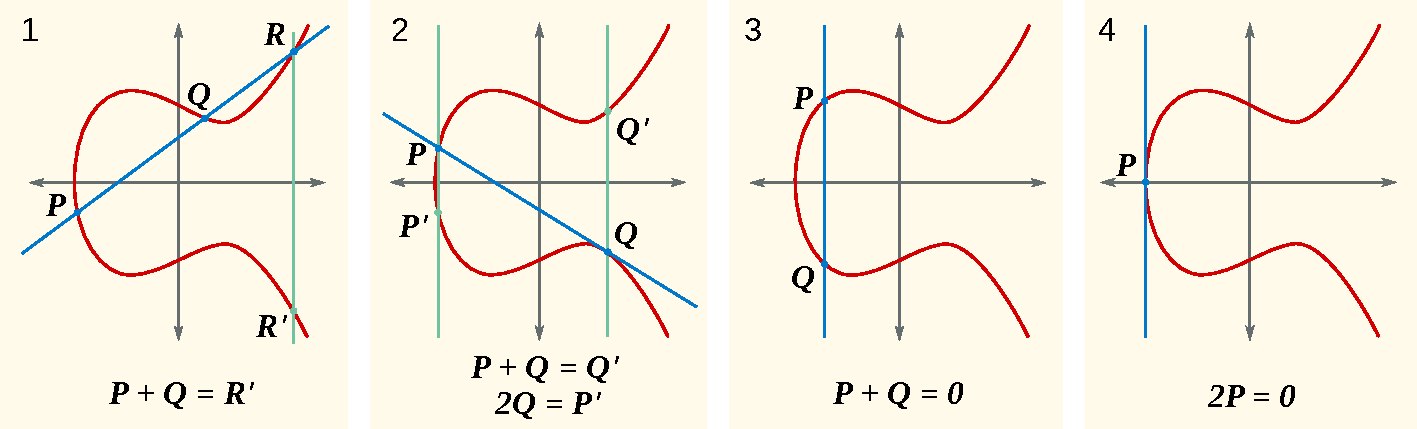
\includegraphics[width=\textwidth]{../thesis/figures/ecc_point_addition.pdf}
    Image by SuperManu, licensed under Creative Commons: \url{https://commons.wikimedia.org/wiki/File:ECClines-2.svg}.
\end{frame}

% \section{Related Research}
\begin{frame}[c]
    \frametitle{Overview of Related Research}
    \begin{center}
        \begin{tikzpicture}[
        xscale=1.25,
        circ/.style={fill, circle, inner sep=1mm},
        lbl_a/.style={align=center, above},
        year_a/.style={align=center, below, yshift=-0.1cm},
        lbl_b/.style={align=center, below},
        year_b/.style={align=center, above, yshift=0.1cm},
    ]

    \draw[dashed, very thick] (-1,0) -- (0,0) (17.25,0) -- ++(0.75,0);
    \draw[very thick] (0,0) -- (17.25, 0);
    
    \draw (1,0) node [circ] {} node [year_a] {2005} -- ++(0, 1) node [lbl_a] {Fuzzy IBE\\First mention of ABE};

    \draw (2,0) node [circ] {} node [year_b] {2006} -- ++(0, -1) node [lbl_b] {First expressive\\ABE scheme};

    \draw (3,0) node [circ] {} node [year_a] {2007} -- ++(0, 2.5) node [lbl_a] {Pairing implementation\\for PC hardware};

    \draw (7, 0) node [circ] {} node [year_b] {2011} -- ++(0, -1) node [lbl_b] {Pairing implementation\\on 8-bit MCU\\(reduced security level)};
    
    \draw (11,0) node [circ] {} node [year_a] {2015} -- ++(0, 1) node [lbl_a] {Pairing-free\\ABE scheme\\\&\\ABE implementation\\on smartphones};

    \draw (12,0) node [circ] {} node [year_b] {2016} -- ++(0, -1) node [lbl_b] {ABE implementation\\on constrained sensor\\\&\\ABE implementation\\on powerful IoT nodes};

    \draw (15,0) node [circ] {} node [year_a] {2019} -- ++(0, 1) node [lbl_a] {Attack on pairing-\\free ABE};

    \draw[color=TUMOrange] (17, 0) node [circ] {} node [year_b] {2021} -- ++(0, -1) node [lbl_b] {This project};

    % \draw (3,0) node 
\end{tikzpicture}
    \end{center}
\end{frame}

\begin{frame}
    \frametitle{Results: Flash use}
    \centering
    \begin{minipage}[h]{\textwidth}\centering
    \pgfplotsset{scaled y ticks=false}
    \begin{tikzpicture}
        \begin{axis}[
            ybar,
            bar shift=0pt,
            ylabel={kilobytes},
            title={Size of executable},
            height=0.7\textheight,
            symbolic x coords={GPSW,YCT},
            xtick={GPSW,YCT},
            ymin=0, ymax=175,
            bar width=2cm,
            enlarge x limits = 0.75,
            nodes near coords,
            every node near coord/.style={
                /pgf/number format/precision=2
            },
        ]
        \addplot[blue, fill=blue!30] coordinates {
            (GPSW, 148.824)
        };
        \addplot[orange, fill=orange!30] coordinates {
            (YCT,	88.288)
        };
        % \addlegendentry{SoC RAM size};
        % \addplot [color=black, mark=none] {262144};
        \end{axis}
    \end{tikzpicture}
\end{minipage}
\end{frame}
%%%%%%%%%%%%%%%%%%%%%%%%%%%%%%%%%%%%%%%%%%%%%%%%%%%%%%%%%%%%%%%%%%%%%%%%%%%%%%%%
\end{document} % !!! NICHT ENTFERNEN !!!
%%%%%%%%%%%%%%%%%%%%%%%%%%%%%%%%%%%%%%%%%%%%%%%%%%%%%%%%%%%%%%%%%%%%%%%%%%%%%%%%

